\section{Arquitetura}

\paragraph{}O projeto desenvolvido se trata de uma aplica��o \textit{Django} que conta com duas interfaces, uma para execu��o de um modelo preditivo em ocorr�ncias controladas e outra para monitoramento do banco de dados, chamadas, respectivamente, de \textit{Showroom} e \textit{Monitor}. Essas duas interfaces s�o controladas pela aplica��o por meio de duas classes de mesmo nome, vistas na figura 3.1.

\begin{figure}
\begin{center}
\parbox[htb]{13.0cm}
  {
  \begin{center}
  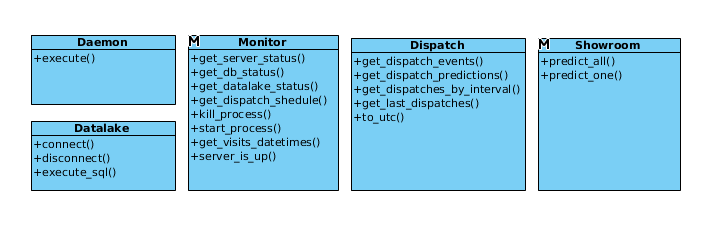
\includegraphics[scale=0.30]{framework_clases.png}
  \caption[\small{Diagrama de classes da aplica��o.}]{\label{FigDel} \small{Diagrama de classes da aplica��o.}}
  \end{center}
  }
\end{center}
\end{figure}

\subsection{Showroom}

\paragraph{}A \textit{view Showroom} � caracterizada pela exist�ncia de casos sobre os quais ser�o inferidas classifica��es a partir do modelo de aprendizado de m�quina carregado na aplica��o. Toda execu��o gerada a partir dessa \textit{view} segue os passos vistos no diagrama de sequ�ncia apresentado na figura 3.2. Os dados para a predi��o s�o coletados, o evento � registrado na tabela de log eventos, o resultado � computado e a \textit{view} � atualizada com os resultados da predi��o.

\begin{figure}
\begin{center}
\parbox[htb]{13.0cm}
  {
  \begin{center}
  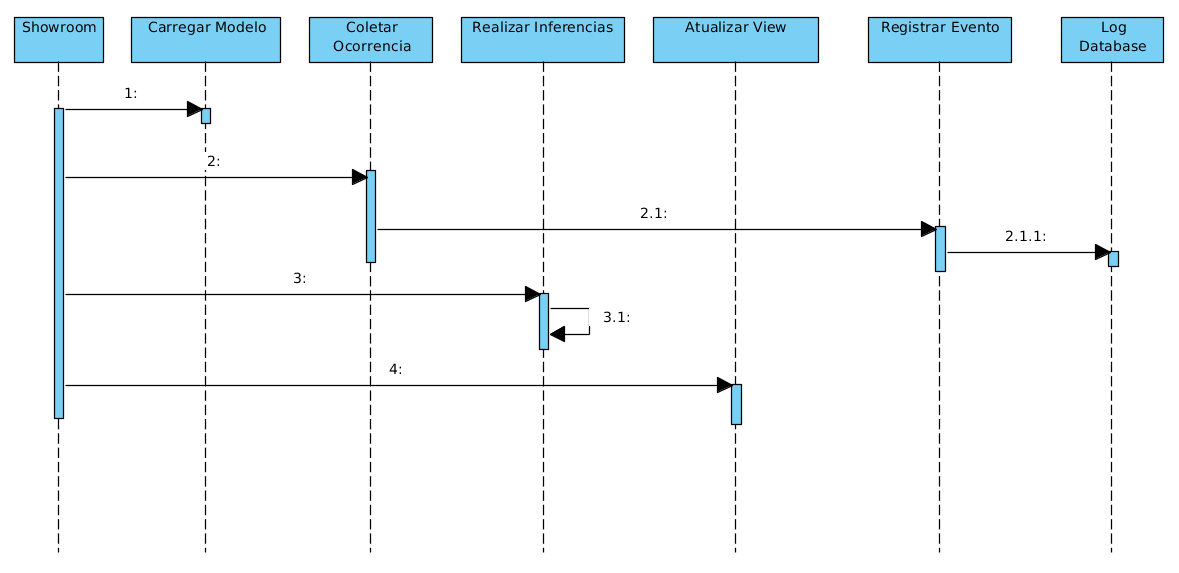
\includegraphics[scale=0.30]{sequence.png}
  \caption[\small{Diagrama de sequ�ncia da \textit{view Showroom}.}]{\label{FigDel} \small{Diagrama de sequ�ncia da \textit{view Showroom}.}}
  \end{center}
  }
\end{center}
\end{figure}

\subsection{Monitor}

\paragraph{}